\documentclass[../main.tex]{subfiles}
\graphicspath{{\subfix{../images}}}


\begin{document}

\subsection{Ricorsione}\label{sec:ricorsione}
Utilizziamo il \textbf{principio di induzione} per mostrare il funzionamento della ricorsione

\begin{exmp}
\begin{equation*}
        S_n = \sum_{k=1}^{n} k = \frac{n * (n+1)}{2}
\end{equation*}

Caso base:
\begin{equation*}
        S_0 = \sum_{k=0}^{0} k = \frac{0 * (0+1)}{2} = 0
\end{equation*}
\end{exmp}

Assumo che $ \mathcal{P} $ valga per $ n $ vado a dimostrare che vale per $n+1$ assunzione:
\begin{equation*}
        S_n = \sum_{k=0}^{n} k = \frac{n * (n+1)}{2}
\end{equation*}
devo dimostrare che 
\begin{equation}\label{eq:induzione_1}
        S_n = \sum_{j=0}^{n+1} j = \frac{n+1 * (n+2)}{2}
\end{equation}
Quindi:        
\begin{equation*}
        S_n = \sum_{k=0}^{n+1} j = \Bigg(\sum_{k=0}^{n} k\Bigg)+ (n+1) = (n+1)\Big(\frac{n+2}{2}\Big)
\end{equation*}
Cosi facendo ho dimostrato~\ref{eq:induzione_1}


\newpage

Altro esempio può essere fatto con i logaritmi, in particolare con:
\begin{equation*}
       \boxed{\log_b x \quad b,x > 0 \quad b \not=1}
\end{equation*}
Dove $ \log_b x $ è quel numero che devo assegnare come esponente a $b$ per ottenere $x$.

\begin{equation*}
        b^y = x
\end{equation*}

\begin{figure}[h!]
        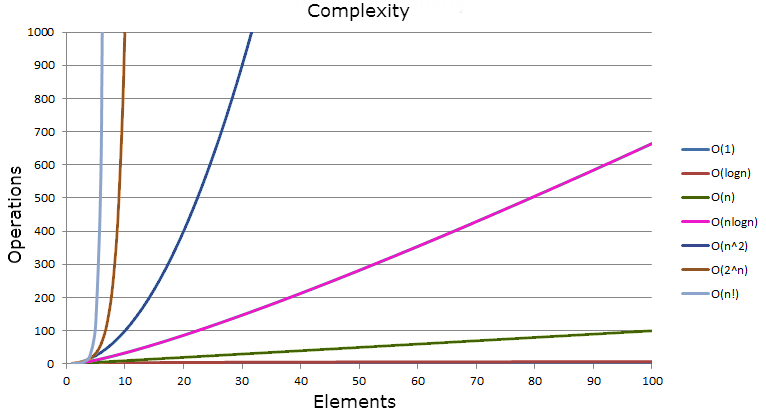
\includegraphics[width=\linewidth]{big-o_complexity.png}
        \caption{Complessità Big-O}
\end{figure}




\end{document}
